\documentclass[tikz,border=5pt]{standalone}

\usepackage{tikz}
\usetikzlibrary{arrows.meta, positioning, calc}

\begin{document}

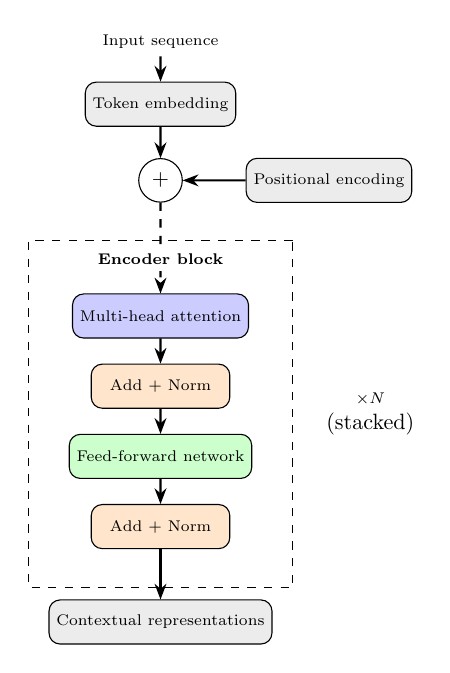
\begin{tikzpicture}[scale=0.8, every node/.style={transform shape},
    block/.style={draw, rounded corners, minimum width=2.2cm, minimum height=0.7cm, align=center},
    thinarrow/.style={-{Stealth[length=2mm,width=1.5mm]}, thick},
    node distance=4mm
]
    % Input tokens
    \node (tok) {\scriptsize Input sequence};
    % Token embedding
    \node[block, fill=gray!15, below=of tok] (emb) {\scriptsize Token embedding};
    % Plus
    \node[draw, circle, below=of emb, yshift=-1mm] (sum) {$+$};
    % Positional encoding
    \node[block, fill=gray!15, right=of sum, xshift=6mm] (posenc) {\scriptsize Positional encoding};

    % Arrows
    \draw[thinarrow] (tok) -- (emb);
    \draw[thinarrow] (emb) -- (sum);
    \draw[thinarrow] (posenc) -- (sum);

    % Encoder block
    \node[below=0.6cm of sum, draw, dashed, inner sep=6pt, minimum height=5.5cm, minimum width=4.2cm] (enc) {};
    
    % Inside encoder
    \node[block, fill=blue!20] at (enc.north) [yshift=-12mm] (mha) {\scriptsize Multi-head attention};
    \node[block, fill=orange!20, below=of mha] (add1) {\scriptsize Add + Norm};
    \node[block, fill=green!20, below=of add1] (ffn) {\scriptsize Feed-forward network};
    \node[block, fill=orange!20, below=of ffn] (add2) {\scriptsize Add + Norm};

    % Arrows
    \draw[thinarrow, dashed] (sum) -- (mha);
    \node[rectangle, fill=white, draw=none, inner sep=3pt] at ($(enc.north)-(0,3mm)$) {\scriptsize\textbf{Encoder block}};
    \draw[thinarrow] (mha) -- (add1);
    \draw[thinarrow] (add1) -- (ffn);
    \draw[thinarrow] (ffn) -- (add2);

    % Stack indication
    \node[right=of enc, align=center] (stack) {\scriptsize $\times N$\\(stacked)};

    % Output
    \node[block, fill=gray!15, below=8mm of add2] (out) {\scriptsize Contextual representations};
    \draw[thinarrow] (add2) -- (out);
\end{tikzpicture}

\end{document}
